\documentclass{article}
\usepackage{fullpage}
\usepackage{brian}
\usepackage{cancel}

\newcommand{\ccancel}[2][black]{\color{#1}\cancel{#2}\normalcolor}
\def\U{\ensuremath{\mathcal{U}}}

\title{Personalized playlist modeling}
\author{Brian McFee}

\begin{document}
\maketitle

\section{Preliminaries}

Let $\U$ denote the set of $m$ users, $\X$ denote the set of $n$ songs, and $\Y$ denote the set of playlists.
Let $\H$ denote an undirected hypergraph over $(\X, \mathcal{E})$, where $\mathcal{E} \subseteq 2^\X$ is the
collection of edges (attribute coincidence).

\section{Personalized model}

The hypergraph random walk model proceeds as follows:
\begin{itemize}
\item select an initial subset $e \in \mathcal{E}$
\item select a song $x$ from $e$
\item select a new subset $e'$ containing $x$
\item go to step 2
\end{itemize}

We add two features to the previous model.  First, a bias term $b_i$ is included to model the global popularity of each
song.  Next, we incorporate a latent factor model to capture individual user preferences for songs.

\subsection{Model equations}

Let $y = (x_0, x_1, \dots, x_T) \in \Y$ denote a playlist, and let $i \in [m]$ index the corresponding user.
The probability of generating $y$ given $u_i$ and the model parameters $\theta \defeq \{u, v, b, w\}$ is defined as follows:
\begin{align*}
\P\left[Y = y \given U = i, \Theta = \theta \right] &= \P\left[X = x_0 \given U = i, \Theta = \theta\right]
\prod_{t=1}^{T} \P\left[X_t = x_t \given X_{t-1}=x_{t-1}, U=i, \Theta=\theta \right]
\end{align*}

The initial edge distribution is characterized as
\begin{align*}
\P\left[E = e \given \Theta = \theta\right] & \defeq \frac{\phantom\sum \exp\{w_e\}}{\displaystyle\sum_{f\in \mathcal{E}} \exp\{w_f\}}
\end{align*}

The probability of drawing a song from a given subset is characterized as
\begin{align*}
\P\left[X_t=x_t \given E=e, U=i, \Theta=\theta \right] &\defeq 
\frac{\phantom\sum\ind{x_t \in e}\exp\left\{u_i\trans v_t + b_t\right\}}{\displaystyle\sum_{j \in \X}\ind{x_j \in e} \exp\left\{u_i\trans v_j + b_j\right\}},
\end{align*}

The bigram transition probability is defined by marginalizing over the edge set $\mathcal{E}$, as follows:
\begin{align*}
\P\left[X_{t}= x_t \given X_{t-1}=x_{t-1}, U=i, \Theta=\theta \right] &\defeq \sum_{e \in \mathcal{E}} 
\P\left[X_{t}=x_t \given E=e, U=i, \Theta=\theta\right]\\
&\phantom{\defeq \sum}\quad\P\left[E=e \given X_{t-1} = x_{t-1}, \Theta=\theta\right]\\
\P\left[E=e \given X_{t-1}=x_{t-1}, \Theta=\theta\right] &\defeq \frac{\phantom\sum\ind{x_{t-1}\in e}\exp\{w_e\}}{ \displaystyle\sum_{f \in \mathcal{E}} \ind{x_{t-1} \in f} \exp\{w_f\} }
\end{align*}

Finally, the model parameters are defined by the following prior distributions
\begin{align*}
u_i &\sim \N(0, \sigma_u I)\\
v_j &\sim \N(0, \sigma_v I)\\
b_j &\sim \N(0, \sigma_b)\\
w_e &\sim \N(0, \sigma_w).\\
\end{align*}

This differs from the previous hypergraph random walk model in that the edge weights are log-normal instead of
exponentially distributed.  \xx{This might work better as a Laplacian distribution.  The same goes for song bias $b_j$.
We'd lose differentiability though.}

Note that all sums over edge membership indicators can be implemented as a dot product against the (sparse, constant) 
song-edge incidence matrix $H \in \{0,1\}^{|\X|, |\mathcal{E}|}$.  If we overload notation, and let $U \in \R^{d\times m}$, $V \in \R^{d \times n}$, $b \in \R^{n}$ and $w \in
\R^{|\mathcal{E}|}$, then the probabilities can be expressed compactly as follows.

\begin{align*}
\P\left[E \given \Theta=\theta\right] &= \frac{\exp\left\{w\right\}}{\one\trans \exp\left\{w\right\}}\\
\P\left[E \given X_{t-1}=x_{t-1}, \Theta=\theta\right] &= \frac{ H_{t-1, \cdot} \odot \exp\left\{w\right\} }{H_{t-1, \cdot}\trans \exp\left\{w\right\}}\\
\P\left[X \given E=e, U=i, \Theta=\theta\right] &= \frac{ H_{\cdot, e} \odot \exp\left\{U_{\cdot,i}\trans V + b\right\} }{ H_{\cdot, e}\trans \exp\left\{U_{\cdot,i}\trans V + b\right\}}
\end{align*}

\begin{figure}
\centering
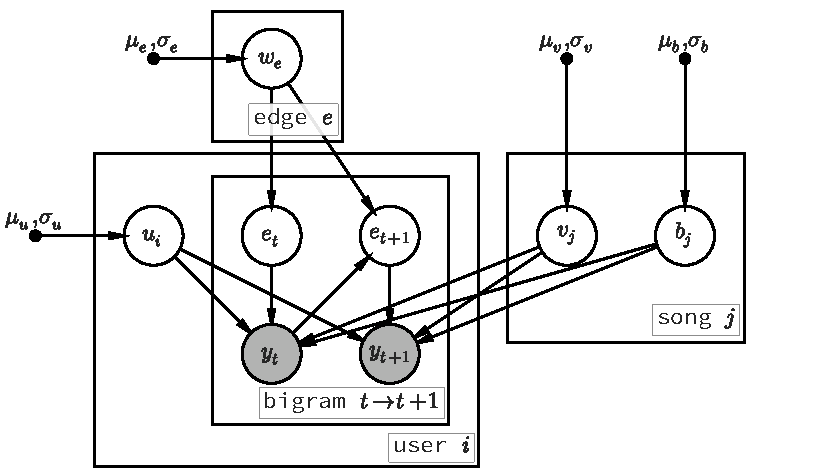
\includegraphics[width=0.7\textwidth]{model}
\caption{Model structure}
\end{figure}

\subsection{Special cases}
The model above generalizes several standard(ish) models directly:
\begin{itemize}
\item Fixing $v_j, b_j$ to zero recovers the original hypergraph model, not counting the repetition constraint and
change of prior.
\item Fixing $v_j$ to zero enables item bias without personalization.
\item Restricting $\mathcal{E} = \{ \X \}$ (\ie, contain only the uniform edge) recovers a simple stochastic latent factor recommender.
\end{itemize}

Note that sampling is relatively efficient if the edge sets are small (on average) and $H$ is sparse.

\section{Parameter estimation}
Given a sample $\Y$, we seek the MAP parameters 
\begin{align*}
\overline{\Theta} \in \argmax_\Theta \P\left[\Theta\given \Y\right] &= \argmax_\Theta \P\left[\Y\given\Theta\right]\P\left[\Theta\right]\\
&= \argmax_\Theta \log \P\left[\Y\given\Theta\right] + \log\P[\Theta]\\
&= \argmax_\Theta \sum_{y\in\Y} \log \P\left[y\given\Theta\right] + \log\P[\Theta]
\end{align*}

The MAP objective is not jointly concave in all parameters $U, V, b, w$.  We will optimize parameters by block coordinate ascent.

\subsection{$U$-step | $V, b, w$ fixed}
The $U$ matrix can be decomposed into its columns, $U = [u_1, u_2, \cdots, u_m]$, where $u_i$ corresponds to the factor for the $i$th user.
Since users are independent, the columns of $u$ can be optimized independently.  Note also that each $u_i$ depends only on the playlists for user $i$.

Let $\Y_i$ denote the playlists of user $i$. The data term for the objective over $u_i$ looks as follows:
\begin{align*}
f(u) &\defeq \sum_{y \in \Y_i} \log\P\left[y\given u_i, V, b, w\right]\\
&= \sum_{y \in \Y_i}\left( \log \P\left[x_0 \given u_i, V, b, w \right] + \sum_{t=1}^T \log \P\left[x_t \given x_{t-1}, u_i, V, b, w \right] \right)
\end{align*}
As noted in the previous section, the initial song likelihood is computed as:
\begin{align*}
\log\P\left[x_0 \given u_i, V, b, w\right] &= \log\sum_{e\in E} \P\left[e\given w\right]\P\left[x_0 \given e, u_i, V, b \right] \\
&= \log\sum_{e\in E} \frac{\exp\{ w_e\}}{\sum_f \exp\{w_f\}} \frac{H_{0, e} \exp\{u_i\trans v_0 + b_0 \} }{H_{\cdot, e}\trans \exp\{u_i\trans V + b \} }\\
&= \log\sum_{e\in E} \exp\{ w_e\} \frac{H_{0, e} \exp\{u_i\trans v_0 + b_0 \} }{H_{\cdot, e}\trans \exp\{u_i\trans V + b \} } - \ccancel[red]{\log\sum_f \exp\{w_f\}}\\
&= \log \exp\{u_i\trans v_0 + b_0 \} \sum_{e \in E} \frac{\exp\{ w_e \} H_{0, e} }{H_{\cdot, e}\trans \exp\{u_i\trans V + b \} }\\
&= u_i\trans v_0 + \ccancel[red]{b_0} + \log \sum_{e\in E}\frac{ H_{0, e}\exp\{w_e\}}{H_{\cdot, e}\trans \exp\{u_i\trans V + b \}}\\
&= u_i\trans v_0 + \log \sum_{e\in E}\frac{ H_{0, e}\exp\{w_e\}}{H_{\cdot, e}\trans \exp\{u_i\trans V + b \}}
\end{align*}
The bigram transition likelihoods are similarly computed:
\begin{align*}
\log\P\left[x_t \given x_{t-1}, u_i, V, b, w\right] &= \log\sum_{e\in E} \P\left[e \given x_{t-1}, w \right]\left[x_t \given e, u_i, V, b \right]\\
&= \log\sum_{e\in E} \frac{H_{t-1,e} \exp\{w_e\} }{H_{t-1,\cdot}\trans \exp\{w\}} \frac{H_{t,e} \exp\{u_i\trans v_t + b_t \} }{H_{\cdot,e}\trans \exp\{u_i\trans V + b \} }\\
&= \log\sum_{e\in E} \frac{H_{t-1,e} \exp\{w_e\} H_{t,e} \exp\{u_i\trans v_t + b_t \} }{H_{\cdot,e}\trans \exp\{u_i\trans V + b \} } - \ccancel[red]{\log H_{t-1,\cdot}\trans
\exp\{w\}}\\
&= u_i\trans v_t + \ccancel[red]{b_t} + \log\sum_{e\in E} \frac{H_{t-1,e} H_{t, e} \exp\{w_e\} }{H_{\cdot,e}\trans \exp\{u_i\trans V + b \} }\\
&= u_i\trans v_t + \log\sum_{e\in E} \frac{H_{t-1,e} H_{t, e} \exp\{w_e\} }{H_{\cdot,e}\trans \exp\{u_i\trans V + b \} }\\
\end{align*}


\subsection{$b$-step | $U, V, w$ fixed}

\subsection{$V$-step | $U, b, w$ fixed}

\subsection{$w$-step | $U, V, b$ fixed}

\end{document}
